% Source: graduate-coursework/Research/Papers/drafts/temporal_context_motion_trails/Radar_TemporalContext_MotionTrails.tex
% Description: Failure mode schematic: long horizons can create a high-density trail region that masks new objects and induces false positives.

\documentclass[border=4pt]{standalone}
\usepackage{algpseudocode}
\usepackage{amsmath,amssymb}
\usepackage[T1]{fontenc}
\usepackage{pgfplots}
\usepackage{tikz}
\usepackage{xcolor}
\pgfplotsset{compat=1.18}
\usetikzlibrary{arrows.meta,positioning,calc,fit,shapes.geometric,shapes.misc,decorations.pathmorphing,backgrounds}


\newcommand{\ph}[1]{\textcolor{red}{#1}}

\begin{document}
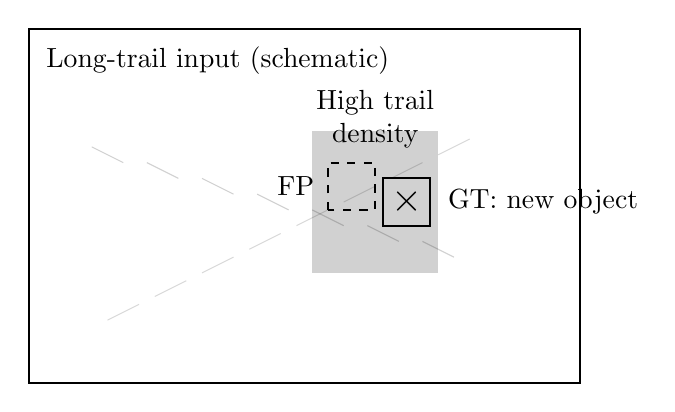
\begin{tikzpicture}[x=1mm,y=1mm]
% Frame boundary
\draw[thick] (0,0) rectangle (70,45);
\node[anchor=north west] at (1,44) {Long-trail input (schematic)};

% Trails
\foreach \k in {0,...,7}{
  \draw[opacity=0.15] (10+\k*6,8+\k*3) -- (14+\k*6,10+\k*3);
}
\foreach \k in {0,...,6}{
  \draw[opacity=0.18] (8+\k*7,30-\k*2) -- (12+\k*7,28-\k*2);
}

% "Stale trail wall"
\fill[opacity=0.18] (36,14) rectangle (52,32);
\node[align=center] at (44,33.5) {High trail\\density};

% New object under clutter
\draw[thick] (45,20) rectangle (51,26);
\node[anchor=west] at (52,23) {GT: new object};

% Spurious detection aligned with trail
\draw[thick, dashed] (38,22) rectangle (44,28);
\node[anchor=east] at (37.5,25) {FP};

% Miss indicator
\draw[thick] (48,23) node {\Large $\times$};

\end{tikzpicture}
\end{document}
